\chapter[Closing Words]{Testing, Analysis and Bench-marking; Closing Remarks, Potential Future Work}
\label{cha:Closing}

\section{Messages, Failures, and Testing in WL} \label{closing:messages}

If WL is to a be a systems engineering language, it makes sense for error cases, failures, to be readily machine readable and conceived of as input for processing in an automated manner, rather than messages that direct a human user of Mathematica Desktop. This shift is apparent in the recommendation for usage of Failure[] rather than the symbol, \lstinline+$Failed+, simply "a special symbol returned by certain functions when they cannot do what they were asked to do." \cite{noauthor_failedwolfram_nodate}

Opposite this, Failure[], introduces more functionality and information, especially the failure type: "Failure[\textit{"tag"},\textit{assoc}] represents a failure of a type indicated by \textit{tag}, with details given by the association assoc." \cite{noauthor_failurewolfram_nodate} This introduces the potential for an abstract way to handle a failure based on type, programmatically, rather than a specific directive.

A basic example of a Failure object is \lstinline+Failure["InvalidInput", <||>]+, without an association even. Inside the Mathematica frontend it is rendered as in figure \ref{fig:simple-failure}.

\begin{figure}[h]
    \centering
    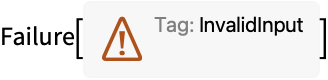
\includegraphics[scale=0.5]{images/closing/O_4.png}
    \caption{A simple Failure object rendered in Mathematica \cite{noauthor_failurewolfram_nodate}}
    \label{fig:simple-failure}
\end{figure}

A more complicated example in terms of metadata and parameterized messaging is generated by the WL code \lstinline$Failure["ExternalOperation", <\|
  "MessageTemplate" -> "External operation `1` failed.", 
  "MessageParameters" -> { "file upload"}\|>]$ and rendered as in figure \ref{fig:templated-failure}.

\begin{figure}[h]
    \centering
    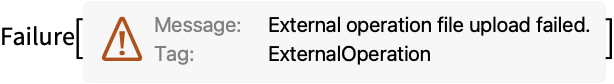
\includegraphics[scale=0.5]{images/closing/O_6.png}
    \caption{A Failure object using a template with positional parameters \cite{noauthor_failurewolfram_nodate}}
    \label{fig:templated-failure}
\end{figure}

Failure can also contain index-able metadata that might be helpful for programmatic retrieval in the failure case. \cite{noauthor_failurewolfram_nodate} In any case, Failure objects can be returned by functions to indicate that an operation did not succeed as expected. This approach allows for more structured error handling, where the calling code can inspect the Failure object to determine the cause of the error and decide how to proceed: They are particularly useful in functional and symbolic programming patterns prevalent in WL, enabling a more nuanced handling of errors compared to traditional imperative error handling mechanisms like throwing exceptions.

Similarly, Message \cite{noauthor_messagewolfram_nodate} is about signaling that something unusual has occurred during the evaluation of an expression - where Failure is a way to encapsulatively represent the occurrence of an error and carry forward information about that error in a structured form, a function might generate a Message to inform the user of an error and then return a Failure object to programmatically indicate the error condition to the calling code.

When a Message is generated, it does not by itself halt execution; the computation continues unless the message is associated with an error severe enough to trigger a termination of the evaluation. \cite{noauthor_messagewolfram_nodate} Messages can be controlled and manipulated using functions like Off, On, and Quiet, allowing to suppress or enable specific messages. This is useful for managing the verbosity of output during computation, especially in cases where certain warnings or errors are expected and do not necessarily indicate a critical failure.

\subsection{Working with Messages in WL}

In WL, messages provide a mechanism for displaying errors, warnings, or other informational text to the user. A message definition typically consists of three parts:

\begin{verbatim}
CloudConnect::creds = "Incorrect username or password.";
\end{verbatim}

The components of a message definition are:

\begin{itemize}
    \item \textbf{Message Head:} The head of a message, such as CloudConnect in the example, represents the function or symbol associated with the message. Some messages are tied to a specific function, while others can be issued by multiple functions. For messages that are generally applicable, the head is set to \texttt{General}. For example:

\begin{verbatim}
General::settf = "Cannot set `1` to `2`; value must be True or False."
\end{verbatim}

    When issuing a message with a \texttt{General} head, the specific function symbol that triggers the message is still used:

\begin{verbatim}
...code...
Message[CloudExpression::settf, dest, expr];
...code...
\end{verbatim}

    \item \textbf{Message Tag:} The message tag is a short, lowercase string that often uses abbreviations. Unlike most naming conventions in the Wolfram Language, message tags do not use camel case or full words. The tag typically alludes to the expected input or operation that was not received or performed correctly.

    \item \textbf{Message Template:} The template is a full sentence that provides the text to be displayed when the message is issued. It can include template slots, which are placeholders (such as \texttt{`1`} or \texttt{`2`}) that will be replaced by data supplied to the Message function at runtime.
\end{itemize}

By using these components, WL allows for standardized, flexible, and informative messaging that enhances user interaction and debugging capabilities.

Usage messages, or message templates, are a way to document the purpose and usage of symbols (typically functions) directly within the WL environment. These messages provide brief descriptions of what a function does, its arguments, and sometimes examples of how to use it. Usage messages are helpful for both package developers and users, as they offer immediate, inline documentation accessible through the WL interface. They are also used in the present package, see near the top of the source code in Appendix \ref{app:Source}.

Testing in WL involves evaluation strategies that check for Messages, or Failures, in the modern case. To this end, the language offers a suite of testing functionality: for example, VerificationTest fails by default if any Message is issued (unless it is told to expect a message, e.g. of a certain type). \cite{wolfram_research_inc_using_2024-1} More recently, TestCreate (\cite{wolfram_research_inc_testcreatewolfram_2024}) and TestEvaluate (\cite{wolfram_research_inc_testevaluatewolfram_2024}) were introduced to the language, to create and run TestObjects, (\cite{noauthor_testobjectwolfram_2024}) respectively.

\subsection{Testing in the Wolfram Language}

WL provides various built-in functions and tools to facilitate different types of testing, including unit tests, integration tests, and performance tests.

\paragraph{Key Features of Testing in WL:}

\begin{itemize}
    \item \textbf{Unit Testing:} WL supports unit testing through the VerificationTest function, which allows developers to specify expected outcomes for individual functions or code blocks. This function compares the actual output against the expected result, making it easy to identify discrepancies.

    \item \textbf{Test Files and Test Framework:} The Wolfram Language has a dedicated testing framework that supports the creation of test files. Test files can contain multiple VerificationTest expressions and are typically stored with a \texttt{.wlt} extension. These test files can be run individually or as part of a suite using the RunTest function.

    \item \textbf{Automatic Test Evaluation:} WL provides tools for automated test evaluation and reporting. TestReport \cite{wolfram_research_inc_testreportwolfram_2024} generates detailed test results, including information on passed, failed, and errored tests. This feature allows developers to quickly assess the overall health of the codebase.

    \item \textbf{Performance Testing:} The Timing and AbsoluteTimingfunctions are used to measure the performance of code in WL. In addition, BenchmarkReport can provide detailed performance analysis, comparing the execution time of different functions or code segments. \cite{wolfram_research_inc_using_2024}

    \item \textbf{Continuous Integration and Testing:} WL integrates well with continuous integration (CI) systems, allowing for automated testing in a CI pipeline - using native WL functionality and, for example, WolframScript \cite{wolfram_research_inc_wolframscriptwolfram_2024} for commandline support - though so-called Testing Notebooks provide an interface for writing and running tests as well \cite{wolfram_research_inc_using_2024-1}
\end{itemize}

The Wolfram Language’s testing framework is designed to provide a robust and flexible environment for developers to ensure the correctness and performance of their code, making it suitable for both small scripts and large-scale projects.

\subsection{Testing Approach for this Project}

For this project, a structured and multi-layered testing approach has been adopted to ensure the reliability and correctness of the code base, which primarily involves converting Theorema notebooks into LaTeX and PDF documents.

\subsubsection{By Testing Category}

The focus from the start was unit testing, however - tests were added towards the end of the project due to an evolving specification (and the work of unearthing the details and the important questions to ask) rather than taking a test-driven approach.

\paragraph{Unit Tests:}

The core functionalities, such as parsing Theorema notebook content, generating \LaTeX files, and handling file operations, are tested in an outside view (irrespective of \LaTeX code quality). These tests  leverage the VerificationTest function to confirm that individual components behave as expected. For instance, the conversion functions like convertToLatexDoc and convertToLatexAndPdfDocs will be tested with various input scenarios to validate their correctness.

The second step is a straightforward unit testing block verifying the expected \LaTeX code of the core parseTmaData function, with a focus on correct rendering of both Theorema Language and Theorema Knowledge.

\paragraph{Integration Tests:}

Integration tests are not performed as part of this project: these would otherwise ensure that the different modules interact correctly. This includes verifying that the file-handling functions correctly create and manipulate LaTeX files, and that the templates are properly filled with data from the Theorema notebooks. Integration testing would also cover the entire conversion workflow, from input notebook to final PDF output: while some coverage through unit testing is provided, these kinds of tests would be left to the Theorema-integration stage.

\paragraph{Performance Tests:}

Performance testing is also not performed as part of this project, due to lack of relevance (time is not considered critical, within rational boundaries). Performance tests would otherwise evaluate the efficiency of the conversion process, particularly for large and complex Theorema notebooks, for instane. Functions like parseTmaData and file generation methods would be profiled using Timing and AbsoluteTiming to identify any potential bottlenecks and ensure optimal performance. \cite{wolfram_research_inc_using_2024-1}

\paragraph{Regression Tests:}

Regression tests will be included to verify that new code changes do not introduce any bugs or negatively affect existing functionality. This will involve re-running all unit and integration tests after any significant code modifications.

\paragraph{Continuous Testing and Automation:}

No continuous integration pipeline or automatic test triggers were created, relying on Mathematica UI solutions, such as Testing Notebooks, for manual testing instead.

\subsubsection{Unknown Pattern Failures}

This failure was initially anticipated for the following case: The central parseTmaData[] recursive function was called with an expression that did not fit any of the expected patterns, falling into the most generic case:

\begin{verbatim}
parseNotebookContent[other_] := StringJoin["\\textcolor{red}{", "Pattern not found! ", ToString[other], "}"]
\end{verbatim}

The manually verifiable output follows the screenshot presented in Image \ref{fig:parseNotebookContent[other_]-output}. Also visible is the run-on output of the string representation of the unmatched pattern printed to the underlying \LaTeX. (The grayed out "Cell reached" and similar directives are used for cross-referencing navigation in the output document back with the origin-document in development.) This approach was finally abandoned in favor of the previously described unit tests comparing the input with a specified output, rather than hinging testing functionality upon the pattern matching process itself.

In the final versions, errors and failures are not actually passed to the output document, and error states hindering evaluation of the main functions simply trigger messages to the user, as described in the opening of this chapter. The generalized approach chosen for parseTmaData and described in the previous chapter relies on the unchaning Theorema Language specification.

\begin{figure}[h]
    \centering
    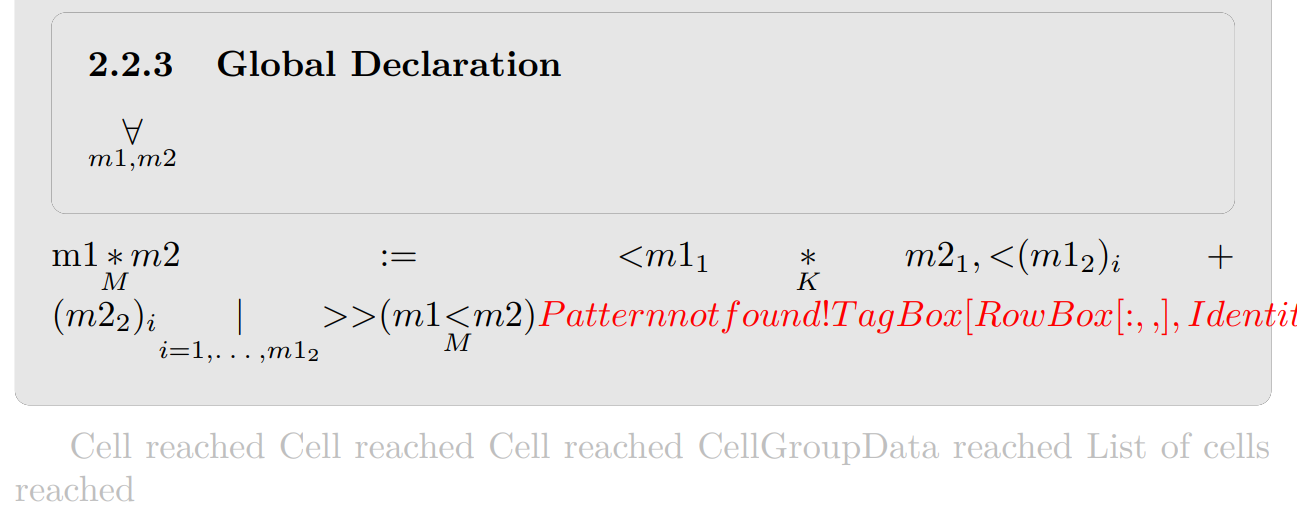
\includegraphics[scale=0.5]{images/closing/Screenshot 2024-03-08 171539.png}
    \caption{parseNotebookContent[other\_] output in document with \LaTeX command formatting}
    \label{fig:parseNotebookContent[other_]-output}
\end{figure}
 
 
\section{Analysis and Review}

The goal of the project was to develop a robust mechanism for transforming Wolfram Language/Theorema notebooks into \LaTeX documents: The transformation logic of the final implementation relied heavily on pattern matching and rule-based programming techniques to accurately map Theorema language constructs to their \LaTeX counterparts. This approach was essential for preserving both the mathematical expressions and structural elements inherent in Theorema notebooks. The solution is designed to integrate seamlessly with the existing Theorema system, utilizing both existing data structures and evaluation mechanisms to achieve a coherent mechanism for translation.

The modular design of the package is a key strength, allowing for straightforward future extensions and modifications. This modularity ensures that additional features or support for more complex Theorema constructs can be incorporated with minimal changes to the existing codebase. 

Review of the FirstTour prototype has confirmed the implementation approach's effectiveness in automating the transformation process. Tests on various Theorema notebook structures demonstrated the accuracy of the \LaTeX output, which faithfully represented the input notebooks, including complex nested formulas and logical constructs. Initial feedback from the main user, the Theorema developer, is positive, highlighting the tool's ability to reduce the manual effort required for \LaTeX preparation significantly. 

In conclusion, the project successfully addressed the initial project objective and provides a functional tool for automating document preparation in Theorema. The project also underscored the potential of Wolfram Language as a versatile tool for software engineering, especially in the context of mathematical document processing: the present work elaborates on the various engineering concepts in this context and presents research on the Wolfram ecosystem extending the language in important ways in the current day. Theorema itself, as a mature WL package and system, provided an ideal entry point to this work.

The project repository, supporting documents, and an introductory exposé of WL are submitted with this thesis.


\section{Final Closing Remarks: Wolfram Language as a Software Engineering Tool and Integrating with Other Languages and Environments, Potential Future Work}

\subsection{Using Wolfram Language for Software Engineering}

This project has demonstrated a use case for mathematical software use, the original domain of Mathematica. In the process of researching and reading the documentation, this researcher discovered a rich ecosystem for WL existing today, including not only integrations with modern enterprise software frameworks, but actually a sophisticated implementation of all the modern software engineering concepts and methodologies, which this work has attempted to demonstrate in structured way.

\subsection{Potential Future Work}

Potential future work hinges on the possible integrations with the native TeXForm functionality, for a more elaborate implementation of a to-\LaTeX typsetting system and less reliance on output-side macros (the \LaTeX template file): possible approaches were sketched out in chapter \ref{cha:Concept}.

Aside from this, the immediately next task to be done is an integration into the Theorema package itself.